% 固定来源 PDF 印刷页 75 第 8 题四组选项函数图象的矢量示意。
% 所有曲线均为定性重绘；曲率、交点精确位置不代表题目给定数据。
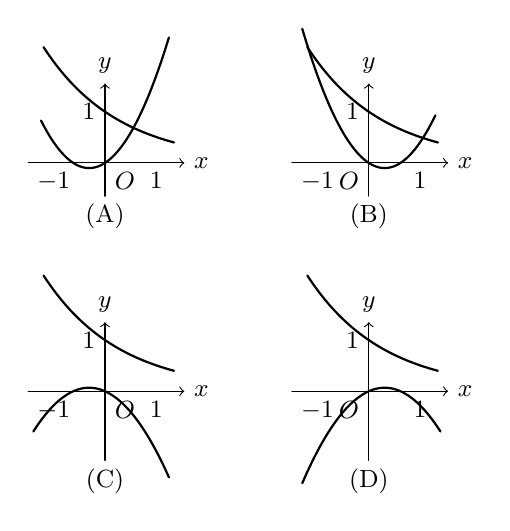
\begin{tikzpicture}[x=.65cm,y=.65cm,font=\small,line cap=round,line join=round]
  \begin{scope}
    \draw[->] (-1.5,0)--(1.55,0) node[right] {$x$};
    \draw[->] (0,-.65)--(0,1.55) node[above] {$y$};
    \draw[thick,domain=-1.25:1.25,samples=60,variable=\x] plot (\x,{1.05*\x*(\x+.62)});
    \draw[thick,domain=-1.2:1.35,samples=60,variable=\x] plot (\x,{exp(-.68*\x)});
    \node[below] at (-1,0) {$-1$}; \node[below right] at (0,0) {$O$}; \node[below] at (1,0) {$1$};
    \node[left] at (0,1) {$1$}; \node at (0,-1.05) {(A)};
  \end{scope}
  \begin{scope}[xshift=3.35cm]
    \draw[->] (-1.5,0)--(1.55,0) node[right] {$x$};
    \draw[->] (0,-.65)--(0,1.55) node[above] {$y$};
    \draw[thick,domain=-1.3:1.3,samples=60,variable=\x] plot (\x,{1.05*\x*(\x-.62)});
    \draw[thick,domain=-1.2:1.35,samples=60,variable=\x] plot (\x,{exp(-.68*\x)});
    \node[below] at (-1,0) {$-1$}; \node[below left] at (0,0) {$O$}; \node[below] at (1,0) {$1$};
    \node[left] at (0,1) {$1$}; \node at (0,-1.05) {(B)};
  \end{scope}
  \begin{scope}[yshift=-2.9cm]
    \draw[->] (-1.5,0)--(1.55,0) node[right] {$x$};
    \draw[->] (0,-1.35)--(0,1.35) node[above] {$y$};
    \draw[thick,domain=-1.4:1.25,samples=60,variable=\x] plot (\x,{-.72*\x*(\x+.62)});
    \draw[thick,domain=-1.2:1.35,samples=60,variable=\x] plot (\x,{exp(-.68*\x)});
    \node[below] at (-1,0) {$-1$}; \node[below right] at (0,0) {$O$}; \node[below] at (1,0) {$1$};
    \node[left] at (0,1) {$1$}; \node at (0,-1.75) {(C)};
  \end{scope}
  \begin{scope}[xshift=3.35cm,yshift=-2.9cm]
    \draw[->] (-1.5,0)--(1.55,0) node[right] {$x$};
    \draw[->] (0,-1.35)--(0,1.35) node[above] {$y$};
    \draw[thick,domain=-1.3:1.4,samples=60,variable=\x] plot (\x,{-.72*\x*(\x-.62)});
    \draw[thick,domain=-1.2:1.35,samples=60,variable=\x] plot (\x,{exp(-.68*\x)});
    \node[below] at (-1,0) {$-1$}; \node[below left] at (0,0) {$O$}; \node[below] at (1,0) {$1$};
    \node[left] at (0,1) {$1$}; \node at (0,-1.75) {(D)};
  \end{scope}
\end{tikzpicture}
